% This file was created by matlab2tikz.
%
%The latest updates can be retrieved from
%  http://www.mathworks.com/matlabcentral/fileexchange/22022-matlab2tikz-matlab2tikz
%where you can also make suggestions and rate matlab2tikz.
%
\definecolor{mycolor1}{rgb}{0.00000,0.44700,0.74100}%
\definecolor{mycolor2}{rgb}{0.92900,0.69400,0.12500}%
\definecolor{mycolor3}{rgb}{0.46600,0.67400,0.18800}%
%
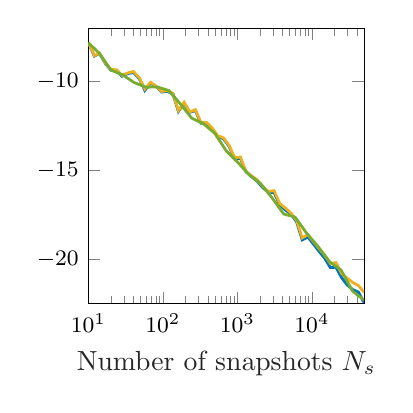
\begin{tikzpicture}

\begin{axis}[%
width=3.5cm,
height=3.5cm,
at={(0.698in,0.577in)},
scale only axis,
xmode=log,
xmin=10,
xmax=50000,
xminorticks=true,
xlabel style={font=\color{white!15!black}},
xlabel={Number of snapshots $N_s$},
ymin=-22.5,
ymax=-7,
ylabel style={font=\color{white!15!black}},
%ylabel={Relative error on diag($\bm{S}_{aa}$) (dB)},
axis background/.style={fill=white},
%legend style={at={(0.03,0.03)}, anchor=south west, legend cell align=left, align=left, fill=none, draw=none},
ticklabel style={font=\footnotesize}
]
\addplot [color=mycolor1, line width=1.0pt]
  table[row sep=crcr]{%
10	-7.82333428697925\\
12	-8.56825865789703\\
14	-8.41307189268658\\
17	-9.00920407597321\\
20	-9.3537297457783\\
24	-9.38154480575806\\
28	-9.69933077355055\\
34	-9.54572626890163\\
40	-9.49363876448267\\
48	-9.83152364928392\\
57	-10.4989520844455\\
68	-10.0885165297253\\
81	-10.289242068753\\
96	-10.5910772256717\\
114	-10.551256659757\\
136	-10.6999195584293\\
161	-11.6822360514168\\
192	-11.2036718289485\\
228	-11.7326383786081\\
272	-11.6321736070583\\
323	-12.3461673158785\\
385	-12.3335241899759\\
458	-12.6797802976475\\
545	-13.1071311573618\\
648	-13.218232503601\\
771	-13.638765374058\\
918	-14.3451312802867\\
1092	-14.3163721616522\\
1299	-15.0794082432676\\
1546	-15.3479160018766\\
1839	-15.6058416506055\\
2189	-15.9796665756589\\
2604	-16.2181576360932\\
3098	-16.2453137480635\\
3687	-16.9325089051901\\
4387	-17.2237873292114\\
5219	-17.445299955056\\
6210	-17.8927718684032\\
7389	-18.9052275179887\\
8792	-18.7444702910516\\
10461	-19.1412845745748\\
12447	-19.5517487895886\\
14810	-19.9365780357358\\
17621	-20.4592505267682\\
20966	-20.4442853610926\\
24947	-21.0280333556023\\
29683	-21.4419733827312\\
35318	-21.7022069388402\\
42022	-21.839653350729\\
50000	-22.4400803719689\\
};
%\addlegendentry{Hald}

\addplot [color=mycolor2, line width=1.0pt]
  table[row sep=crcr]{%
10	-7.80793444781493\\
12	-8.54357234510443\\
14	-8.39469514057678\\
17	-8.98371296425242\\
20	-9.3101201341527\\
24	-9.34059800029062\\
28	-9.64825236997246\\
34	-9.51225679351986\\
40	-9.43386375730012\\
48	-9.77951121147543\\
57	-10.4193291725435\\
68	-10.0379120952645\\
81	-10.2573112531791\\
96	-10.5586968410626\\
114	-10.5084519556703\\
136	-10.6607374022787\\
161	-11.6366904050299\\
192	-11.1646612483853\\
228	-11.7090090135855\\
272	-11.5828455868267\\
323	-12.3119340391412\\
385	-12.2961968775694\\
458	-12.6139941963631\\
545	-13.0462003552294\\
648	-13.164294408213\\
771	-13.5852880495537\\
918	-14.2886191897588\\
1092	-14.240923911883\\
1299	-15.0626456778487\\
1546	-15.3070545686674\\
1839	-15.5220368679069\\
2189	-15.9174132191443\\
2604	-16.1826401774589\\
3098	-16.1347602952486\\
3687	-16.8636455530214\\
4387	-17.1103588814124\\
5219	-17.3923233267944\\
6210	-17.808185727603\\
7389	-18.7954459777261\\
8792	-18.6127800084382\\
10461	-19.0080069318031\\
12447	-19.3990249536675\\
14810	-19.7751973105429\\
17621	-20.2296220421925\\
20966	-20.1802510326307\\
24947	-20.7961953526922\\
29683	-21.0595998378458\\
35318	-21.3013727638665\\
42022	-21.473265640537\\
50000	-21.8618900925979\\
};
%\addlegendentry{Basic AP}

\addplot [color=mycolor3, line width=1.0pt]
  table[row sep=crcr]{%
10	-7.82333428699501\\
14	-8.41307189274591\\
20	-9.35372974578693\\
29	-9.63226374349065\\
41	-10.056806638212\\
59	-10.3160387339534\\
84	-10.3049677497188\\
120	-10.5051609432566\\
171	-11.2595840432922\\
244	-12.0640998211784\\
348	-12.3633902035622\\
496	-12.9177426253893\\
707	-13.8970601211009\\
1008	-14.5430890893978\\
1438	-15.2498805656574\\
2050	-15.7474277967298\\
2924	-16.5527174272982\\
4170	-17.4486278403843\\
5946	-17.6268302116185\\
8479	-18.5343612923237\\
12091	-19.2863256678069\\
17242	-20.1388078820684\\
24588	-20.6028943537641\\
35063	-21.790971614331\\
50000	-22.2895980979102\\
};
%\addlegendentry{Dougherty}

\end{axis}
\end{tikzpicture}%